\chapter{Kreuzkorrelation und Faltung}
\section{Einführung Kreuzkorrelation}
Die Kreuzkorrelation wird verwendet, um die Korrelation zwischen zwei Signalen oder Sequenzen zu berechnen. Dabei werden unterschiedliche Zeitverschiebungen zwischen
den Sequenzen eingesetzt. NumPy verwendet dabei folgende Formel für die 
Kreuzkorrelation\footnote{Siehe: Dokumentation NumPy:\cite{DocumentationNumpyCorrelate} und Definition Kreuzkorrelation: \cite{DefinitionCrossCorrelation}.}.

\[
  f \star g \equiv \int\limits_{-\infty}^{+\infty} \overline{f}(-t)*g(t)
\]
Die Formel kann in eine Form umgewandelt werden, aus der die Verschiebung einer Sequenz gegenüber einer anderen besser ersichtlich 
ist\footnote{Umformung: siehe: \cite{DefinitionCrossCorrelation}.}:
\[
  f \star g \equiv \int\limits_{-\infty}^{+\infty} \overline{f}(-\tau)*g(t + \tau) \text{ } \mathrm{d}\tau
\]

NumPy bietet dabei unterschiedliche Modi bei der Berechnung der Kreuzkorrelation an. Diese entsprechen den Modi der mathematischen Faltung ( zu Englisch \enquote{Convolution}).
Die Unterschiede der Kreuzkorrelation und Faltung sowie der Autokorrelation sind in den folgenden Abbildungen dargestellt.
Abbildung~\ref{fig:compareConvulationCrosscorrelationAutoCorrelation} bietet einen Überblick, während die Abbildungen~\ref{fig:convolutionExample1} und \ref{fig:convolutionExample2} animiert sind.
Sollte die Animation nicht korrekt dargestellt werden, sind diese über die jeweilige Quellenangaben einsehbar.

\section{Beispiele Kreuzkorrelation, Faltung und Autokorrelation}
\begin{figure}[H]
  \centering
  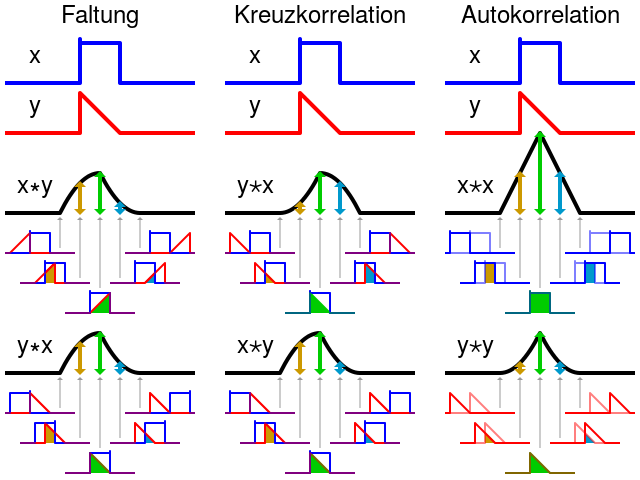
\includegraphics[width=0.8\linewidth]{./images/comparisonConvolutionCorrelation.png}
  \caption[Vergleich zwischen Faltung, Kreuzkorrelation und Autokorrelation]{Vergleicht die Faltung, Kreuzkorrelation und Autokorrelation\footnotemark}
  \label{fig:compareConvulationCrosscorrelationAutoCorrelation}
\end{figure}
\footnotetext{Quelle: \cite[]{CompareConvulationCrosscorrelationAutoCorrelation}}

\begin{figure}[H]
  \centering
  \animategraphics[loop,autoplay,label=convolutionExample1]{25}{./images/convolutionExample1/frame_}{1}{301}
  \caption[Animation: Beispiel 1 für die Faltung]{Darstellung einer eindimensionalen Faltung\footnotemark}
  \label{fig:convolutionExample1}
\end{figure}
\footnotetext{Quelle: \cite[]{ConvultionExample1Wikimedia}}

\begin{figure}[H]
  \centering
  \animategraphics[loop,autoplay]{25}{./images/convolutionExample2/frame_}{1}{161}
  \caption[Animation: Beispiel 2 für die Faltung]{Faltung zweier Gaussfunktionen\footnotemark}
  \label{fig:convolutionExample2}
\end{figure}
\footnotetext{Quelle: \cite[]{ConvultionExample2Wikimedia}}

\section{Bedeutung der unterschiedlichen Modi}
\begin{samepage}
  In den Beschreibungen gelten folgende Voraussetzungen: 
  \begin{align*}
    & \text{Sequenz A: von }a[0] \text{ bis }a[L_A - 1] \text{ mit } L_A = \text{Länge von Sequenz A}\\
    & \text{Sequenz A: von }b[0] \text{ bis }b[L_B - 1] \text{ mit } L_B = \text{Länge von Sequenz B}
  \end{align*}
  Als Quelle dient die Dokumentation\footnote{Dokumentation NumPy Correlate: \cite{DocumentationNumpyCorrelate}.} sowie eine Beschreibung der 
  Modi\footnote{Beschreibung der Modi: \cite{NumPyCorrelationModesExplained}.}.
\end{samepage}


\subsection{Modus: Valid}
Dieser Modus wird verwendet, wenn der Modus nicht explizit angegeben wird.\\
Dabei wird eine Ausgabe der Länge $ max(L_A, L_B) - min(L_A, L_B) + 1 $ erzeugt. Die Verschiebung findet dabei im Bereich 
von $ min(L_A, L_B) - 1 \text{ bis } - max(L_A, L_B) - 1 $ statt.

\subsection{Modus: Full}
In diesem Modus wird die Berechnung im Bereich von $ 0 \text{ bis }  L_A + L_B - 2 $ durchgeführt. 
Dadurch ergibt sich eine Ausgabe von $ L_A + L_B + 1 $ Elementen. Dabei können Effekte an den Rändern der Sequenzen auftreten, da diese
sich dort nicht mehr voll überlappen.

\subsection{Modus: Same}
Liefert ein Ergebnis der Länge $ max(L_A, L_B) $ . Dabei können ebenfalls Effekte an den Rändern auftreten.\\
Die Berechnug findet im Bereich von $ \frac{(L_B - 1)}{2} \text{ bis } L_A - 1 + \frac{L_B - 1}{2} $ statt. \\
Sollte $ L_A < L_B $ gelten, werden die beiden Sequenzen vor der Berechnung ausgetauscht.










